% Figure 2: Cylindrical Cavity with Axial Field
% Author: Dr. Computernonymouse
% Description: Cylindrical resonant cavity showing longitudinal standing waves
%              and transverse field patterns for directional ZPE extraction

\documentclass[tikz,border=10pt]{standalone}
\usepackage{tikz}
\usepackage{tikz-3dplot}
\usepackage{pgfplots}
\usepackage{amsmath}
\usepackage{amssymb}

\pgfplotsset{compat=1.18}
\usetikzlibrary{arrows.meta,patterns,decorations.markings,calc,backgrounds,shadings,3d}

% Define colors
\definecolor{cavitywall}{RGB}{120,120,120}
\definecolor{fieldblue}{RGB}{31,119,180}
\definecolor{fieldred}{RGB}{214,39,40}
\definecolor{wavevector}{RGB}{255,127,14}
\definecolor{standingwave}{RGB}{148,103,189}

\begin{document}

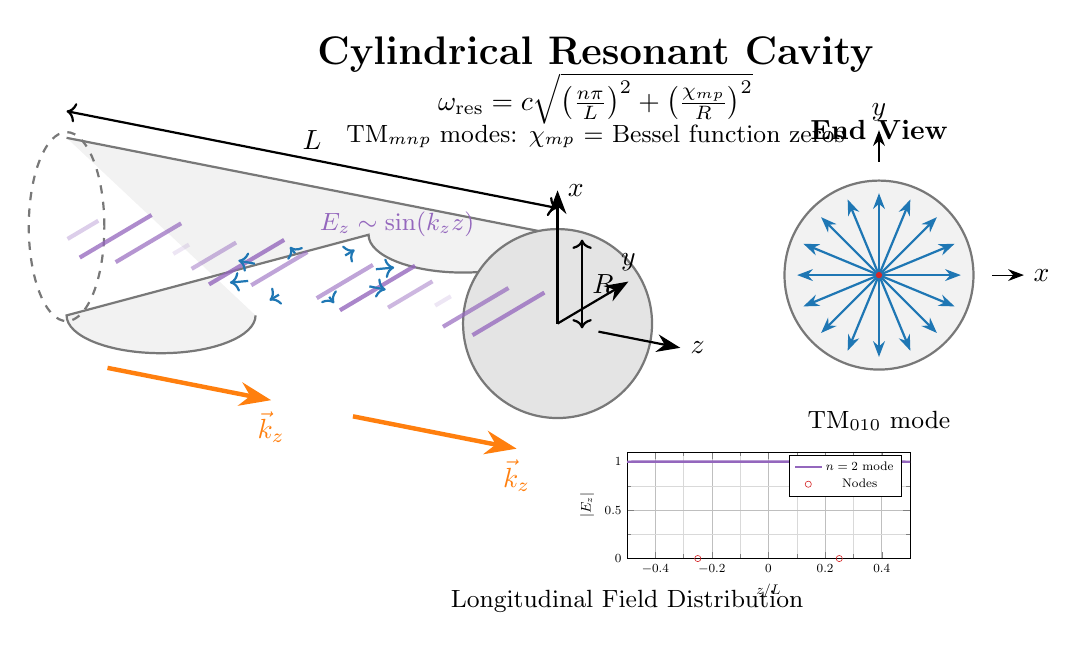
\begin{tikzpicture}[scale=0.8]

% Main view: 3D perspective of cylindrical cavity
\begin{scope}[shift={(0,0)}]
    \tdplotsetmaincoords{70}{30}
    \begin{scope}[tdplot_main_coords,scale=1.5]

        % Draw cylinder body
        \draw[thick,cavitywall,fill=cavitywall!10]
            (-3,0,1) -- (3,0,1) arc (0:-180:1cm and 0.4cm) -- (-3,0,-1) arc (180:360:1cm and 0.4cm);

        % Front end cap
        \draw[thick,cavitywall,fill=cavitywall!20]
            (3,0,0) ellipse (1cm and 1cm);

        % Back end cap (dashed for transparency)
        \draw[thick,cavitywall,dashed]
            (-3,0,0) ellipse (0.4cm and 1cm);

        % Standing wave pattern along z-axis
        \foreach \z in {-2.8,-2.4,...,2.8} {
            \pgfmathsetmacro{\amplitude}{sin(\z*180/1.5)}
            \pgfmathsetmacro{\opacity}{abs(\amplitude)*80}
            \draw[standingwave,opacity=\opacity/100,line width=1.5pt]
                (\z,-0.8*\amplitude,0) -- (\z,0.8*\amplitude,0);
        }

        % Wavevector arrows
        \draw[-{Stealth[length=4mm]},wavevector,ultra thick]
            (-2.5,0,-1.5) -- (-0.5,0,-1.5) node[below] {$\vec{k}_z$};
        \draw[-{Stealth[length=4mm]},wavevector,ultra thick]
            (0.5,0,-1.5) -- (2.5,0,-1.5) node[below] {$\vec{k}_z$};

        % Transverse field lines (circular)
        \foreach \angle in {0,45,90,135,180,225,270,315} {
            \draw[fieldblue,thick,->]
                ({0.7*cos(\angle)},{0.7*sin(\angle)},0) -- ({0.9*cos(\angle)},{0.9*sin(\angle)},0);
        }

        % Axis labels
        \draw[-{Stealth[length=3mm]},black,thick] (3.5,0,0) -- (4.5,0,0) node[right] {$z$};
        \draw[-{Stealth[length=3mm]},black,thick] (3,0,0) -- (3,1.5,0) node[above] {$y$};
        \draw[-{Stealth[length=3mm]},black,thick] (3,0,0) -- (3,0,1.5) node[right] {$x$};

        % Dimension labels
        \draw[<->,thick] (-3,0,1.3) -- (3,0,1.3) node[midway,above] {$L$};
        \draw[<->,thick] (3.3,0,0) -- (3.3,0,1) node[midway,right] {$R$};

        % Mode label
        \node[standingwave,font=\small] at (0,1.8,0) {$E_z \sim \sin(k_z z)$};

    \end{scope}
\end{scope}

% Side view: Cross-section showing field pattern
\begin{scope}[shift={(9,0)}]
    % Draw circular cross-section
    \draw[thick,cavitywall,fill=cavitywall!10] (0,0) circle (1.5cm);

    % Radial field lines
    \foreach \angle in {0,22.5,45,67.5,90,112.5,135,157.5,180,202.5,225,247.5,270,292.5,315,337.5} {
        \draw[fieldblue,thick,-{Stealth[length=2mm]}]
            (0,0) -- ({1.3*cos(\angle)},{1.3*sin(\angle)});
    }

    % Center point
    \fill[fieldred] (0,0) circle (0.05cm);

    % Labels
    \node[above,font=\bfseries] at (0,2) {End View};
    \node[below,font=\small] at (0,-2) {TM$_{010}$ mode};

    % Coordinate indicators
    \draw[-{Stealth[length=2mm]},black] (1.8,0) -- (2.3,0) node[right] {$x$};
    \draw[-{Stealth[length=2mm]},black] (0,1.8) -- (0,2.3) node[above] {$y$};
\end{scope}

% Longitudinal field distribution plot
\begin{scope}[shift={(5,-4.5)},scale=0.7]
    \begin{axis}[
        width=8cm,
        height=4cm,
        xlabel={$z/L$},
        ylabel={$|E_z|$},
        xmin=-0.5,xmax=0.5,
        ymin=0,ymax=1.1,
        grid=both,
        grid style={line width=0.3pt, draw=gray!30},
        major grid style={line width=0.5pt,draw=gray!50},
        minor tick num=1,
        xlabel style={font=\small},
        ylabel style={font=\small},
        tick label style={font=\footnotesize},
        legend pos=north east,
        legend style={font=\footnotesize}
    ]

    % Standing wave pattern
    \addplot[standingwave,ultra thick,smooth,samples=100,domain=-0.5:0.5]
        {abs(cos(2*pi*x))};
    \addlegendentry{$n=2$ mode}

    % Node positions
    \addplot[only marks,mark=o,mark size=2pt,fieldred]
        coordinates {(-0.25,0) (0.25,0)};
    \addlegendentry{Nodes}

    \end{axis}

    \node[below,font=\small] at (0,-0.5) {Longitudinal Field Distribution};
\end{scope}

% Title and resonance condition
\node[font=\Large\bfseries] at (4.5,3.5) {Cylindrical Resonant Cavity};
\node[font=\normalsize] at (4.5,2.8) {$\omega_{\text{res}} = c\sqrt{\left(\frac{n\pi}{L}\right)^2 + \left(\frac{\chi_{mp}}{R}\right)^2}$};
\node[font=\small] at (4.5,2.2) {TM$_{mnp}$ modes: $\chi_{mp}$ = Bessel function zeros};

\end{tikzpicture}

\end{document}